\hypertarget{Distributions_8c}{
\section{Distributions.c File Reference}
\label{Distributions_8c}\index{Distributions.c@{Distributions.c}}
}
{\tt \#include \char`\"{}party.h\char`\"{}}\par


Include dependency graph for Distributions.c:\nopagebreak
\begin{figure}[H]
\begin{center}
\leavevmode
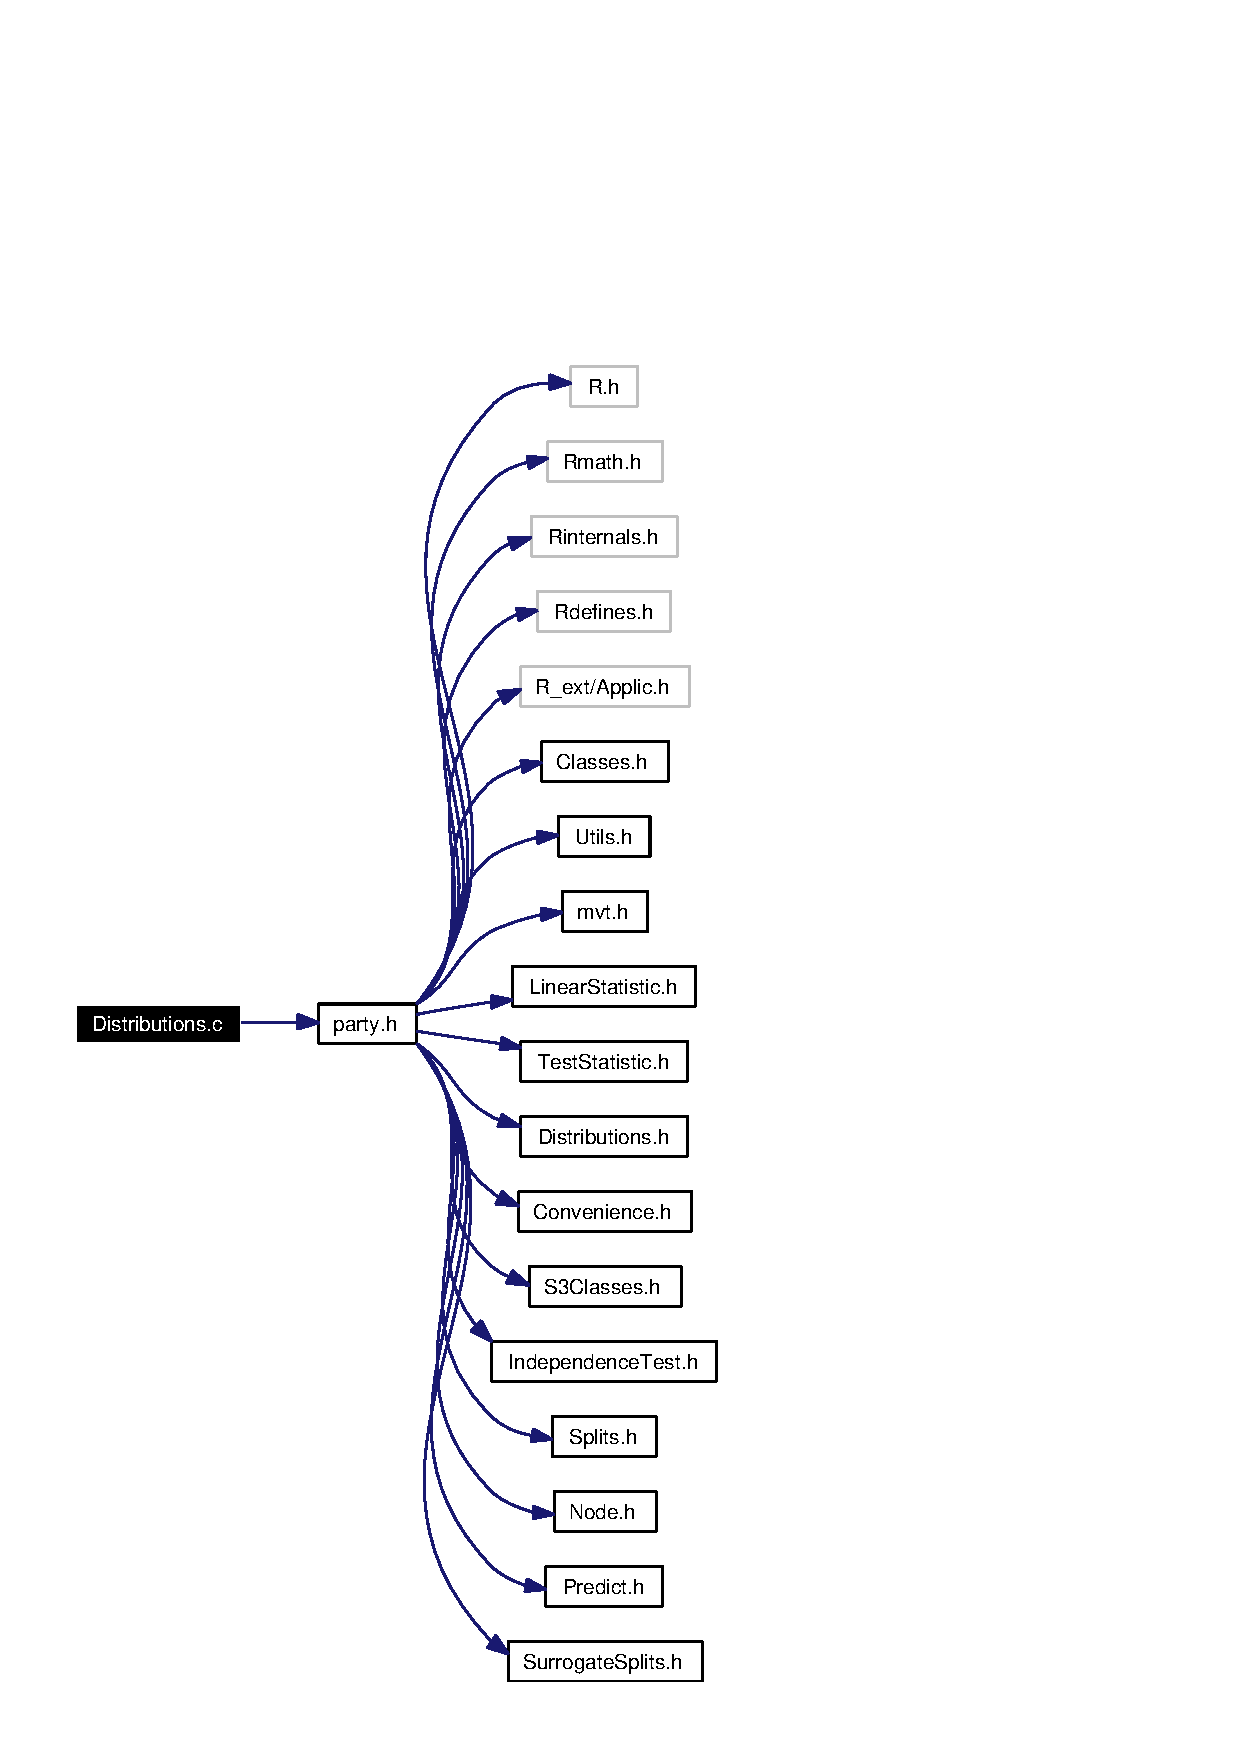
\includegraphics[width=420pt]{Distributions_8c__incl}
\end{center}
\end{figure}
\subsection*{Functions}
\begin{CompactItemize}
\item 
double \hyperlink{Distributions_8c_a692392488ab88e95a62d2142e9d428c}{C\_\-quadformConditionalPvalue} (const double tstat, const double df)
\item 
SEXP \hyperlink{Distributions_8c_f9d46ed74aa1e81c94ddbfdbf5cf504f}{R\_\-quadformConditionalPvalue} (SEXP tstat, SEXP df)
\item 
double \hyperlink{Distributions_8c_0b0373aa22dcf8b8ecf6b9c560db9c70}{C\_\-maxabsConditionalPvalue} (const double tstat, const double $\ast$Sigma, const int pq, int $\ast$maxpts, double $\ast$releps, double $\ast$abseps, double $\ast$tol)
\item 
SEXP \hyperlink{Distributions_8c_23e23063d2a1c5ecfb6e1603d0edc228}{R\_\-maxabsConditionalPvalue} (SEXP tstat, SEXP Sigma, SEXP maxpts, SEXP releps, SEXP abseps, SEXP tol)
\item 
void \hyperlink{Distributions_8c_662bfb70585ca9948ff29d7ed370273b}{C\_\-MonteCarlo} (double $\ast$criterion, SEXP learnsample, SEXP weights, SEXP fitmem, SEXP varctrl, SEXP gtctrl, double $\ast$ans\_\-pvalues)
\item 
SEXP \hyperlink{Distributions_8c_06bd58bb395eb700a056db4498c4db9c}{R\_\-MonteCarlo} (SEXP criterion, SEXP learnsample, SEXP weights, SEXP fitmem, SEXP varctrl, SEXP gtctrl)
\end{CompactItemize}


\subsection{Detailed Description}
Conditional Distributions

\begin{Desc}
\item[Author:]\begin{Desc}
\item[Author]\end{Desc}
\end{Desc}
\begin{Desc}
\item[Date:]\begin{Desc}
\item[Date]\end{Desc}
\end{Desc}


Definition in file \hyperlink{Distributions_8c-source}{Distributions.c}.

\subsection{Function Documentation}
\hypertarget{Distributions_8c_0b0373aa22dcf8b8ecf6b9c560db9c70}{
\index{Distributions.c@{Distributions.c}!C_maxabsConditionalPvalue@{C\_\-maxabsConditionalPvalue}}
\index{C_maxabsConditionalPvalue@{C\_\-maxabsConditionalPvalue}!Distributions.c@{Distributions.c}}
\subsubsection{\setlength{\rightskip}{0pt plus 5cm}double C\_\-maxabsConditionalPvalue (const double {\em tstat}, const double $\ast$ {\em Sigma}, const int {\em pq}, int $\ast$ {\em maxpts}, double $\ast$ {\em releps}, double $\ast$ {\em abseps}, double $\ast$ {\em tol})}}
\label{Distributions_8c_0b0373aa22dcf8b8ecf6b9c560db9c70}


Conditional asymptotic P-value of a maxabs-type test statistic\par
 Basically the functionality from package `mvtnorm' \par
 \begin{Desc}
\item[Parameters:]
\begin{description}
\item[{\em tstat}]test statitstic \item[{\em Sigma}]covariance matrix \item[{\em pq}]nrow(Sigma) \item[{\em maxpts}]number of Monte-Carlo steps \item[{\em releps}]relative error \item[{\em abseps}]absolute error \item[{\em tol}]tolerance \end{description}
\end{Desc}


Definition at line 52 of file Distributions.c.

Referenced by C\_\-ConditionalPvalue(), and R\_\-maxabsConditionalPvalue().\hypertarget{Distributions_8c_662bfb70585ca9948ff29d7ed370273b}{
\index{Distributions.c@{Distributions.c}!C_MonteCarlo@{C\_\-MonteCarlo}}
\index{C_MonteCarlo@{C\_\-MonteCarlo}!Distributions.c@{Distributions.c}}
\subsubsection{\setlength{\rightskip}{0pt plus 5cm}void C\_\-MonteCarlo (double $\ast$ {\em criterion}, SEXP {\em learnsample}, SEXP {\em weights}, SEXP {\em fitmem}, SEXP {\em varctrl}, SEXP {\em gtctrl}, double $\ast$ {\em ans\_\-pvalues})}}
\label{Distributions_8c_662bfb70585ca9948ff29d7ed370273b}


Monte-Carlo approximation to the conditional pvalues \begin{Desc}
\item[Parameters:]
\begin{description}
\item[{\em criterion}]vector of node criteria for each input \item[{\em learnsample}]an object of class `LearningSample' \item[{\em weights}]case weights \item[{\em fitmem}]an object of class `TreeFitMemory' \item[{\em varctrl}]an object of class `VariableControl' \item[{\em gtctrl}]an object of class `GlobalTestControl' \item[{\em ans\_\-pvalues}]return values; vector of adjusted pvalues \end{description}
\end{Desc}


Definition at line 169 of file Distributions.c.

Referenced by C\_\-GlobalTest(), and R\_\-MonteCarlo().\hypertarget{Distributions_8c_a692392488ab88e95a62d2142e9d428c}{
\index{Distributions.c@{Distributions.c}!C_quadformConditionalPvalue@{C\_\-quadformConditionalPvalue}}
\index{C_quadformConditionalPvalue@{C\_\-quadformConditionalPvalue}!Distributions.c@{Distributions.c}}
\subsubsection{\setlength{\rightskip}{0pt plus 5cm}double C\_\-quadformConditionalPvalue (const double {\em tstat}, const double {\em df})}}
\label{Distributions_8c_a692392488ab88e95a62d2142e9d428c}


Conditional asymptotic P-value of a quadratic form\par
 \begin{Desc}
\item[Parameters:]
\begin{description}
\item[{\em tstat}]test statistic \item[{\em df}]degree of freedom \end{description}
\end{Desc}


Definition at line 18 of file Distributions.c.

Referenced by C\_\-ConditionalPvalue(), and R\_\-quadformConditionalPvalue().\hypertarget{Distributions_8c_23e23063d2a1c5ecfb6e1603d0edc228}{
\index{Distributions.c@{Distributions.c}!R_maxabsConditionalPvalue@{R\_\-maxabsConditionalPvalue}}
\index{R_maxabsConditionalPvalue@{R\_\-maxabsConditionalPvalue}!Distributions.c@{Distributions.c}}
\subsubsection{\setlength{\rightskip}{0pt plus 5cm}SEXP R\_\-maxabsConditionalPvalue (SEXP {\em tstat}, SEXP {\em Sigma}, SEXP {\em maxpts}, SEXP {\em releps}, SEXP {\em abseps}, SEXP {\em tol})}}
\label{Distributions_8c_23e23063d2a1c5ecfb6e1603d0edc228}


R-interface to C\_\-maxabsConditionalPvalue \par
 \begin{Desc}
\item[Parameters:]
\begin{description}
\item[{\em tstat}]test statitstic \item[{\em Sigma}]covariance matrix \item[{\em maxpts}]number of Monte-Carlo steps \item[{\em releps}]relative error \item[{\em abseps}]absolute error \item[{\em tol}]tolerance \end{description}
\end{Desc}


Definition at line 142 of file Distributions.c.

References C\_\-maxabsConditionalPvalue(), and nrow().

Here is the call graph for this function:\nopagebreak
\begin{figure}[H]
\begin{center}
\leavevmode
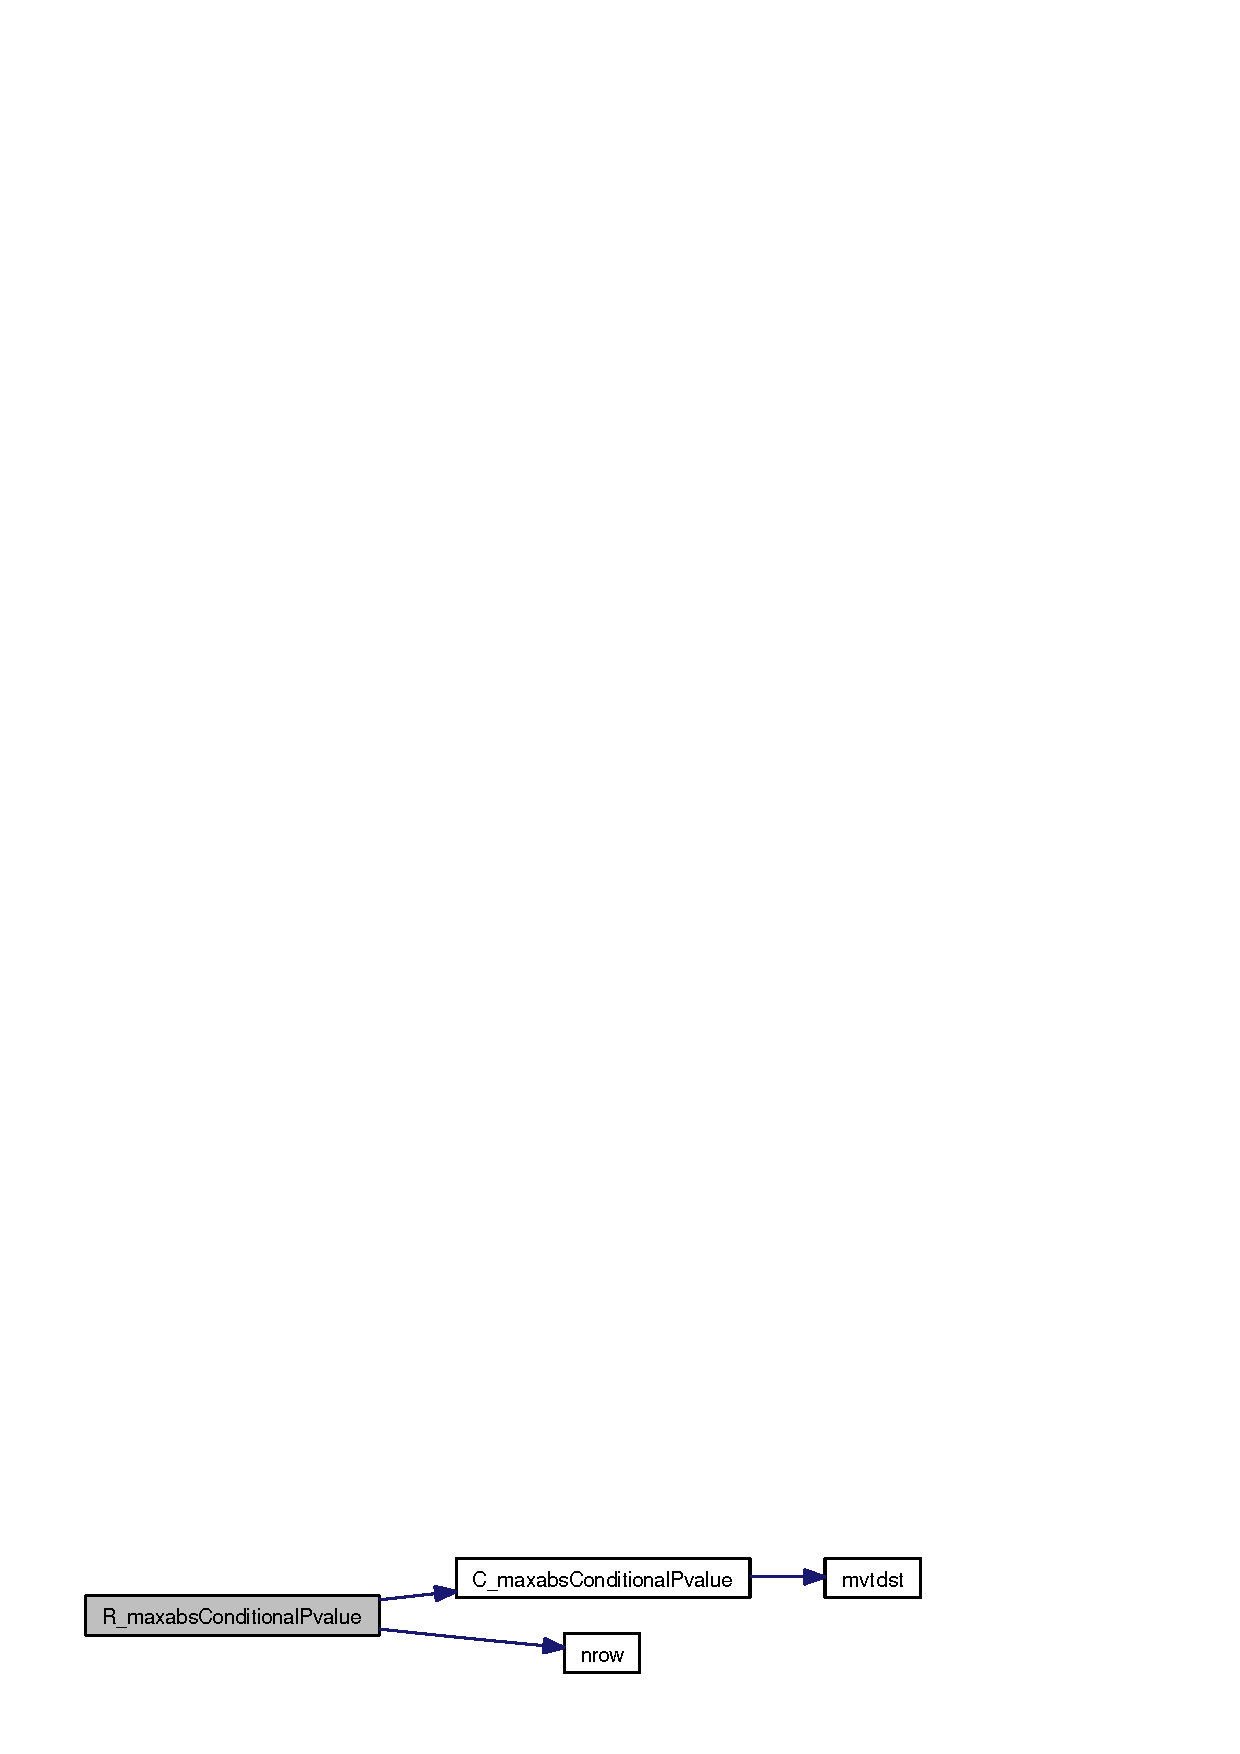
\includegraphics[width=195pt]{Distributions_8c_23e23063d2a1c5ecfb6e1603d0edc228_cgraph}
\end{center}
\end{figure}
\hypertarget{Distributions_8c_06bd58bb395eb700a056db4498c4db9c}{
\index{Distributions.c@{Distributions.c}!R_MonteCarlo@{R\_\-MonteCarlo}}
\index{R_MonteCarlo@{R\_\-MonteCarlo}!Distributions.c@{Distributions.c}}
\subsubsection{\setlength{\rightskip}{0pt plus 5cm}SEXP R\_\-MonteCarlo (SEXP {\em criterion}, SEXP {\em learnsample}, SEXP {\em weights}, SEXP {\em fitmem}, SEXP {\em varctrl}, SEXP {\em gtctrl})}}
\label{Distributions_8c_06bd58bb395eb700a056db4498c4db9c}


R-interface to C\_\-MonteCarlo \par
 \begin{Desc}
\item[Parameters:]
\begin{description}
\item[{\em criterion}]vector of node criteria for each input \item[{\em learnsample}]an object of class `LearningSample' \item[{\em weights}]case weights \item[{\em fitmem}]an object of class `TreeFitMemory' \item[{\em varctrl}]an object of class `VariableControl' \item[{\em gtctrl}]an object of class `GlobalTestControl' \end{description}
\end{Desc}


Definition at line 278 of file Distributions.c.

References C\_\-MonteCarlo(), and get\_\-ninputs().

Here is the call graph for this function:\nopagebreak
\begin{figure}[H]
\begin{center}
\leavevmode
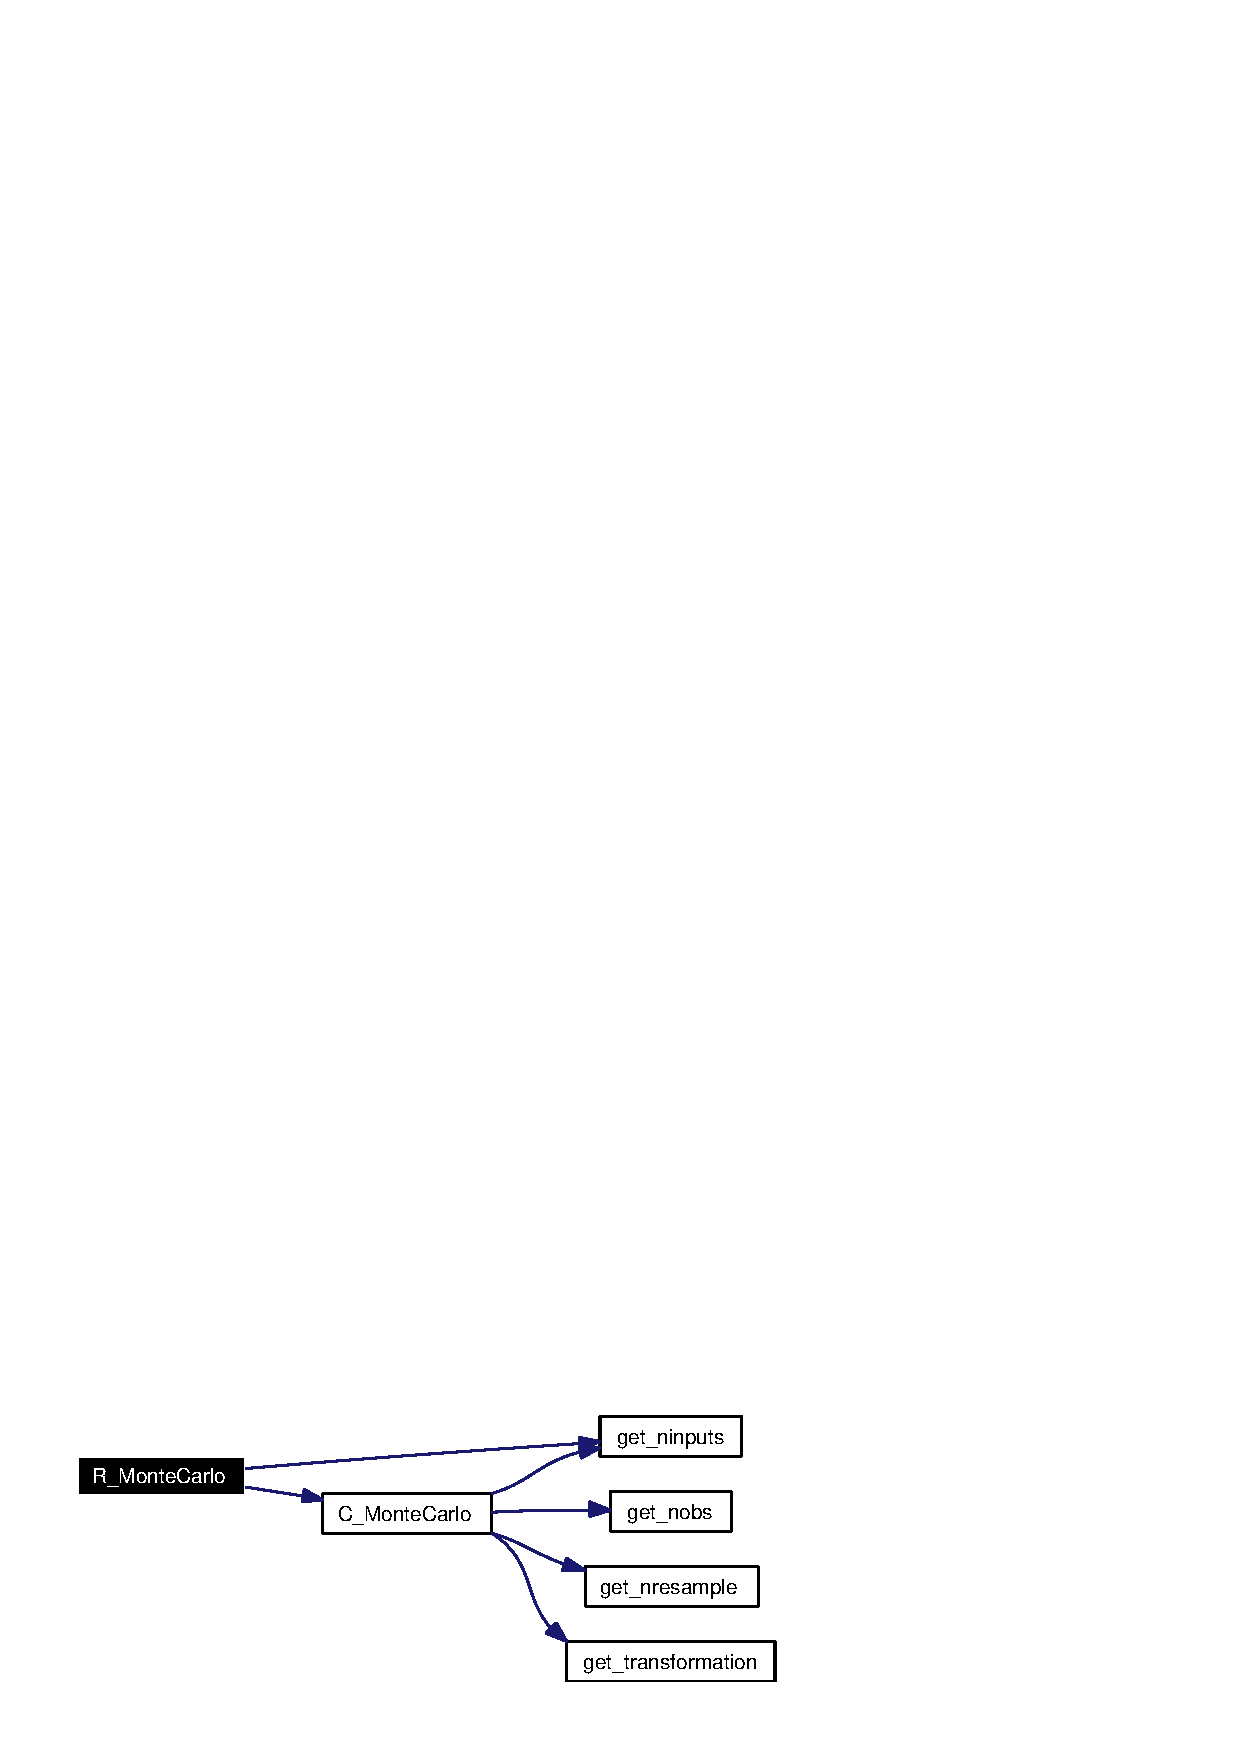
\includegraphics[width=126pt]{Distributions_8c_06bd58bb395eb700a056db4498c4db9c_cgraph}
\end{center}
\end{figure}
\hypertarget{Distributions_8c_f9d46ed74aa1e81c94ddbfdbf5cf504f}{
\index{Distributions.c@{Distributions.c}!R_quadformConditionalPvalue@{R\_\-quadformConditionalPvalue}}
\index{R_quadformConditionalPvalue@{R\_\-quadformConditionalPvalue}!Distributions.c@{Distributions.c}}
\subsubsection{\setlength{\rightskip}{0pt plus 5cm}SEXP R\_\-quadformConditionalPvalue (SEXP {\em tstat}, SEXP {\em df})}}
\label{Distributions_8c_f9d46ed74aa1e81c94ddbfdbf5cf504f}


R-interface to C\_\-quadformConditionalPvalue\par
 \begin{Desc}
\item[Parameters:]
\begin{description}
\item[{\em tstat}]test statitstic \item[{\em df}]degree of freedom \end{description}
\end{Desc}


Definition at line 29 of file Distributions.c.

References C\_\-quadformConditionalPvalue().

Here is the call graph for this function:\nopagebreak
\begin{figure}[H]
\begin{center}
\leavevmode

\includegraphics[width=204pt]{Distributions_8c_f9d46ed74aa1e81c94ddbfdbf5cf504f_cgraph}
\end{center}
\end{figure}
